% Introductory concepts; grounded in the verified L4 trace where indicated.
\section{Coding agent basics}
\sectionframe{01}{How a coding\\agent works}

\begin{frame}{A coding agent acts, observes, and tries again}
\tagline{A large language model (LLM) predicts text and structured tool requests.}

\begin{tikzpicture}
\path[use as bounding box] (0,-2.5) rectangle (13.35,.4);
\node[fill=teal!8,rounded corners=2mm,minimum width=3.6cm,minimum height=1.7cm,align=center] (model) at (1.9,-.8)
{\emoji[7mm]{robot}\\[1mm]\textbf{Model}};
\node[fill=orange!10,rounded corners=2mm,minimum width=3.6cm,minimum height=1.7cm,align=center] (tools) at (11.2,-.8)
{\emoji[7mm]{tools}\\[1mm]\textbf{Tools}};
\draw[flow link,draw=teal] (3.8,-.3)--node[above=1.5mm,font=\small]{Request an action}(9.3,-.3);
\draw[flow link,draw=orange] (9.3,-1.3)--node[below=1.5mm,font=\small]{Return a result}(3.8,-1.3);
\end{tikzpicture}

\vspace{2mm}
\begin{columns}[T,onlytextwidth]
\column{.48\textwidth}\eyebrow[teal]{THE MODEL DECIDES}
\small Which file looks relevant? What should change?
\column{.48\textwidth}\eyebrow{TOOLS DO THE WORK}
\small Search, read files, edit code, and run tests.
\end{columns}
\vspace{2mm}
\takeaway{During a repair, the model reads new results; its learned parameters stay fixed.}

\note{The model receives the issue, instructions, and previous observations. It can generate a structured tool request. The agent runtime validates and executes that request in the allowed environment, then returns the result to the model. The language model does not directly execute a command merely by mentioning it in text. Each iteration consumes context, time, and sometimes a tool-call budget.}
\end{frame}

\begin{frame}{A tool call, shown as a conversation}
\tagline{From our completed run: the agent is looking for the URL highlighter.}
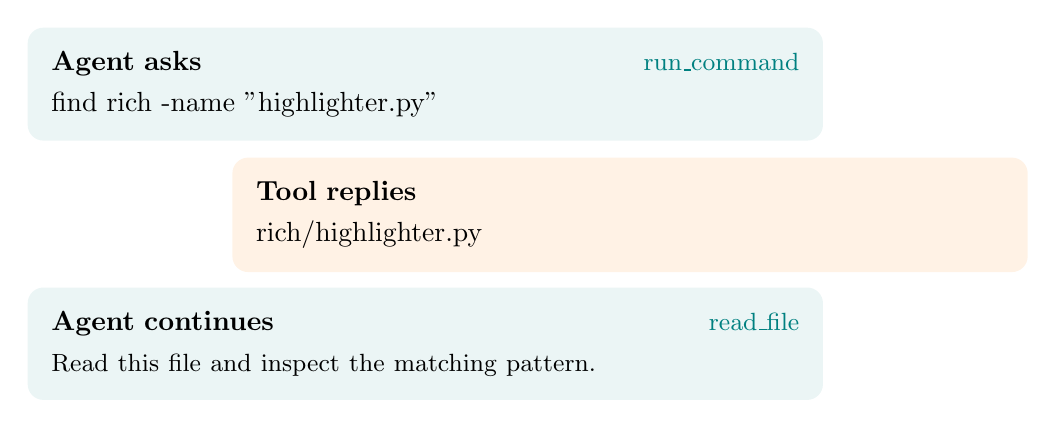
\begin{tikzpicture}
\node[anchor=north west,fill=teal!8,rounded corners=2mm,inner sep=3mm,text width=9.5cm,align=left] (a) at (0,0)
{\textbf{Agent asks} \hfill {\small\color{teal}run\_command}\\[1mm]
\pathcode{find rich -name "highlighter.py"}};
\node[anchor=north west,fill=orange!10,rounded corners=2mm,inner sep=3mm,text width=9.5cm,align=left] (b) at (2.6,-1.65)
{\textbf{Tool replies}\\[1mm]\pathcode{rich/highlighter.py}};
\node[anchor=north west,fill=teal!8,rounded corners=2mm,inner sep=3mm,text width=9.5cm,align=left] (c) at (0,-3.3)
{\textbf{Agent continues} \hfill {\small\color{teal}read\_file}\\[1mm]
\small Read this file and inspect the matching pattern.};
\end{tikzpicture}
% Sources: runs/kaggle-runtime-smoke/kaggle-output/runtime-smoke/infer/results/traces/trace_rich_3454.json, steps 3 and 4.
\note{This is a faithful excerpt from the first two tool actions in the rich 3454 L4 trace. The actual request contains a function name and a command argument; the result contains stdout, stderr, and exit code. The next request uses read\_file with the returned path. The shell command finds a filename; it does not repair anything. File inspection, editing, and tests follow as separate actions.}
\end{frame}

\begin{frame}{One small repair makes the loop concrete}
\tagline{Public task \texttt{rich\_3454}; the URL below illustrates the bug.}
\begin{columns}[T,onlytextwidth]
\column{.48\textwidth}
\softpanel{teal}{Before the fix}{
The match stops before @.\par\vspace{3mm}
\texttt{\textcolor{teal}{https://example.com/}\underline{@user}}}
\column{.48\textwidth}
\softpanel{orange}{After the fix}{
The whole URL is highlighted.\par\vspace{3mm}
\texttt{\textcolor{orange}{https://example.com/\underline{@user}}}}
\end{columns}
\vspace{2mm}
\eyebrow{EDIT, CHECK, FINISH}
\small Allow @ in the matching pattern and add a regression test.\par\vspace{2mm}
\pathcode{pytest tests/test_highlighter.py}\quad$\longrightarrow$\quad\textbf{Tests pass}\par\vspace{2mm}
\small The agent finishes and exports a patch: its changes as a Git diff.
% Sources: rich_3454 issue and downloaded L4 prediction/trace; URL on this slide is illustrative.
\note{The public issue explicitly points to the highlighter and the missing character, so this is a useful introductory example but not evidence that every hidden issue is equally easy. The displayed URL is illustrative. The actual agent changed rich/highlighter.py and added a regression test. Kaggle's independent verification is separate from tests the agent chooses to run while working. The completed-run slide later reports the actual tests and public score.}
\end{frame}
